% Options for packages loaded elsewhere
\PassOptionsToPackage{unicode}{hyperref}
\PassOptionsToPackage{hyphens}{url}
%
\documentclass[
]{article}
\title{Pesticide Labels Now Report}
\usepackage{etoolbox}
\makeatletter
\providecommand{\subtitle}[1]{% add subtitle to \maketitle
  \apptocmd{\@title}{\par {\large #1 \par}}{}{}
}
\makeatother
\subtitle{Draft}
\author{}
\date{\vspace{-2.5em}2022-03-18}

\usepackage{amsmath,amssymb}
\usepackage{lmodern}
\usepackage{iftex}
\ifPDFTeX
  \usepackage[T1]{fontenc}
  \usepackage[utf8]{inputenc}
  \usepackage{textcomp} % provide euro and other symbols
\else % if luatex or xetex
  \usepackage{unicode-math}
  \defaultfontfeatures{Scale=MatchLowercase}
  \defaultfontfeatures[\rmfamily]{Ligatures=TeX,Scale=1}
\fi
% Use upquote if available, for straight quotes in verbatim environments
\IfFileExists{upquote.sty}{\usepackage{upquote}}{}
\IfFileExists{microtype.sty}{% use microtype if available
  \usepackage[]{microtype}
  \UseMicrotypeSet[protrusion]{basicmath} % disable protrusion for tt fonts
}{}
\makeatletter
\@ifundefined{KOMAClassName}{% if non-KOMA class
  \IfFileExists{parskip.sty}{%
    \usepackage{parskip}
  }{% else
    \setlength{\parindent}{0pt}
    \setlength{\parskip}{6pt plus 2pt minus 1pt}}
}{% if KOMA class
  \KOMAoptions{parskip=half}}
\makeatother
\usepackage{xcolor}
\IfFileExists{xurl.sty}{\usepackage{xurl}}{} % add URL line breaks if available
\IfFileExists{bookmark.sty}{\usepackage{bookmark}}{\usepackage{hyperref}}
\hypersetup{
  pdftitle={Pesticide Labels Now Report},
  hidelinks,
  pdfcreator={LaTeX via pandoc}}
\urlstyle{same} % disable monospaced font for URLs
\usepackage[margin=1in]{geometry}
\usepackage{color}
\usepackage{fancyvrb}
\newcommand{\VerbBar}{|}
\newcommand{\VERB}{\Verb[commandchars=\\\{\}]}
\DefineVerbatimEnvironment{Highlighting}{Verbatim}{commandchars=\\\{\}}
% Add ',fontsize=\small' for more characters per line
\usepackage{framed}
\definecolor{shadecolor}{RGB}{248,248,248}
\newenvironment{Shaded}{\begin{snugshade}}{\end{snugshade}}
\newcommand{\AlertTok}[1]{\textcolor[rgb]{0.94,0.16,0.16}{#1}}
\newcommand{\AnnotationTok}[1]{\textcolor[rgb]{0.56,0.35,0.01}{\textbf{\textit{#1}}}}
\newcommand{\AttributeTok}[1]{\textcolor[rgb]{0.77,0.63,0.00}{#1}}
\newcommand{\BaseNTok}[1]{\textcolor[rgb]{0.00,0.00,0.81}{#1}}
\newcommand{\BuiltInTok}[1]{#1}
\newcommand{\CharTok}[1]{\textcolor[rgb]{0.31,0.60,0.02}{#1}}
\newcommand{\CommentTok}[1]{\textcolor[rgb]{0.56,0.35,0.01}{\textit{#1}}}
\newcommand{\CommentVarTok}[1]{\textcolor[rgb]{0.56,0.35,0.01}{\textbf{\textit{#1}}}}
\newcommand{\ConstantTok}[1]{\textcolor[rgb]{0.00,0.00,0.00}{#1}}
\newcommand{\ControlFlowTok}[1]{\textcolor[rgb]{0.13,0.29,0.53}{\textbf{#1}}}
\newcommand{\DataTypeTok}[1]{\textcolor[rgb]{0.13,0.29,0.53}{#1}}
\newcommand{\DecValTok}[1]{\textcolor[rgb]{0.00,0.00,0.81}{#1}}
\newcommand{\DocumentationTok}[1]{\textcolor[rgb]{0.56,0.35,0.01}{\textbf{\textit{#1}}}}
\newcommand{\ErrorTok}[1]{\textcolor[rgb]{0.64,0.00,0.00}{\textbf{#1}}}
\newcommand{\ExtensionTok}[1]{#1}
\newcommand{\FloatTok}[1]{\textcolor[rgb]{0.00,0.00,0.81}{#1}}
\newcommand{\FunctionTok}[1]{\textcolor[rgb]{0.00,0.00,0.00}{#1}}
\newcommand{\ImportTok}[1]{#1}
\newcommand{\InformationTok}[1]{\textcolor[rgb]{0.56,0.35,0.01}{\textbf{\textit{#1}}}}
\newcommand{\KeywordTok}[1]{\textcolor[rgb]{0.13,0.29,0.53}{\textbf{#1}}}
\newcommand{\NormalTok}[1]{#1}
\newcommand{\OperatorTok}[1]{\textcolor[rgb]{0.81,0.36,0.00}{\textbf{#1}}}
\newcommand{\OtherTok}[1]{\textcolor[rgb]{0.56,0.35,0.01}{#1}}
\newcommand{\PreprocessorTok}[1]{\textcolor[rgb]{0.56,0.35,0.01}{\textit{#1}}}
\newcommand{\RegionMarkerTok}[1]{#1}
\newcommand{\SpecialCharTok}[1]{\textcolor[rgb]{0.00,0.00,0.00}{#1}}
\newcommand{\SpecialStringTok}[1]{\textcolor[rgb]{0.31,0.60,0.02}{#1}}
\newcommand{\StringTok}[1]{\textcolor[rgb]{0.31,0.60,0.02}{#1}}
\newcommand{\VariableTok}[1]{\textcolor[rgb]{0.00,0.00,0.00}{#1}}
\newcommand{\VerbatimStringTok}[1]{\textcolor[rgb]{0.31,0.60,0.02}{#1}}
\newcommand{\WarningTok}[1]{\textcolor[rgb]{0.56,0.35,0.01}{\textbf{\textit{#1}}}}
\usepackage{longtable,booktabs,array}
\usepackage{calc} % for calculating minipage widths
% Correct order of tables after \paragraph or \subparagraph
\usepackage{etoolbox}
\makeatletter
\patchcmd\longtable{\par}{\if@noskipsec\mbox{}\fi\par}{}{}
\makeatother
% Allow footnotes in longtable head/foot
\IfFileExists{footnotehyper.sty}{\usepackage{footnotehyper}}{\usepackage{footnote}}
\makesavenoteenv{longtable}
\usepackage{graphicx}
\makeatletter
\def\maxwidth{\ifdim\Gin@nat@width>\linewidth\linewidth\else\Gin@nat@width\fi}
\def\maxheight{\ifdim\Gin@nat@height>\textheight\textheight\else\Gin@nat@height\fi}
\makeatother
% Scale images if necessary, so that they will not overflow the page
% margins by default, and it is still possible to overwrite the defaults
% using explicit options in \includegraphics[width, height, ...]{}
\setkeys{Gin}{width=\maxwidth,height=\maxheight,keepaspectratio}
% Set default figure placement to htbp
\makeatletter
\def\fps@figure{htbp}
\makeatother
\setlength{\emergencystretch}{3em} % prevent overfull lines
\providecommand{\tightlist}{%
  \setlength{\itemsep}{0pt}\setlength{\parskip}{0pt}}
\setcounter{secnumdepth}{-\maxdimen} % remove section numbering
\usepackage{booktabs}
\usepackage{longtable}
\usepackage{array}
\usepackage{multirow}
\usepackage{wrapfig}
\usepackage{float}
\usepackage{colortbl}
\usepackage{pdflscape}
\usepackage{tabu}
\usepackage{threeparttable}
\usepackage{threeparttablex}
\usepackage[normalem]{ulem}
\usepackage{makecell}
\usepackage{xcolor}
\ifLuaTeX
  \usepackage{selnolig}  % disable illegal ligatures
\fi

\begin{document}
\maketitle

{
\setcounter{tocdepth}{4}
\tableofcontents
}
\hypertarget{executive-summary}{%
\section{Executive Summary}\label{executive-summary}}

A data dictionary and descriptive statistics were prepared based on the
Pesticide Labels Now (PLN)
\href{https://docs.google.com/document/d/1mUHPYdpWljCWroODGenUjYlyae2ZWwqN4MScBLXlr2U/edit}{analysis
plan}. For a better representation of users, we ignored a list of random
identifiers (`aid' in \emph{ignores.csv}) associated with the project
team members and generated descriptive statistics for three subsets:

\begin{itemize}
\tightlist
\item
  evDownload.01
\item
  evStart
\item
  evViewPage.01
\end{itemize}

\hypertarget{data-dictionary}{%
\section{Data Dictionary}\label{data-dictionary}}

\hypertarget{evdownload.01-subset}{%
\subsection{evDownload.01 subset}\label{evdownload.01-subset}}

Unique devices (aid)

\begin{Shaded}
\begin{Highlighting}[]
\FunctionTok{print}\NormalTok{(}\FunctionTok{n\_distinct}\NormalTok{(evDownload}\FloatTok{.01}\SpecialCharTok{$}\NormalTok{aid), }\AttributeTok{style=}\StringTok{"rmarkdown"}\NormalTok{)}
\end{Highlighting}
\end{Shaded}

\begin{verbatim}
## [1] 93
\end{verbatim}

\begin{longtable}[]{@{}ll@{}}
\toprule
Variable & Description \\
\midrule
\endhead
aid & Random device identifier \\
epaReg & EPA regsistration number \\
prodName & Pesticide product name \\
sourcePage & App page visited? \\
evType & Action taken on app (download) \\
ts & Timestamp yyy:mm:dd:hh:mm:ss \\
\bottomrule
\end{longtable}

\hypertarget{evstart-subset}{%
\subsection{evStart subset}\label{evstart-subset}}

Unique users (aid)

\begin{Shaded}
\begin{Highlighting}[]
\FunctionTok{print}\NormalTok{(}\FunctionTok{n\_distinct}\NormalTok{(evStart}\SpecialCharTok{$}\NormalTok{aid), }\AttributeTok{style=}\StringTok{"rmarkdown"}\NormalTok{)}
\end{Highlighting}
\end{Shaded}

\begin{verbatim}
## [1] 392
\end{verbatim}

\begin{longtable}[]{@{}ll@{}}
\toprule
Variable & Description \\
\midrule
\endhead
aid & Random device identifier \\
evDesc1 & App version? \\
evDesc2 & Device type \\
evDesc3 & GPS coordinates \\
evType & Action taken on app (start page) \\
ts & Timestamp yyy:mm:dd:hh:mm:ss \\
\bottomrule
\end{longtable}

\hypertarget{evviewpage.01-subset}{%
\subsection{evViewPage.01 subset}\label{evviewpage.01-subset}}

Unique users (aid)

\begin{Shaded}
\begin{Highlighting}[]
\FunctionTok{print}\NormalTok{(}\FunctionTok{n\_distinct}\NormalTok{(evViewPage}\FloatTok{.01}\SpecialCharTok{$}\NormalTok{aid), }\AttributeTok{style=}\StringTok{"rmarkdown"}\NormalTok{)}
\end{Highlighting}
\end{Shaded}

\begin{verbatim}
## [1] 358
\end{verbatim}

\begin{longtable}[]{@{}ll@{}}
\toprule
Variable & Description \\
\midrule
\endhead
aid & Random device identifier \\
evDesc1 & First action on app \\
evDesc2 & English or Spanish \\
evDesc3 & Pesticide label viewed \\
evType & Action taken on app (view page) \\
ts & Timestamp yyy:mm:dd:hh:mm:ss \\
\bottomrule
\end{longtable}

\hypertarget{detailed-variable-descriptions}{%
\subsection{Detailed variable
descriptions}\label{detailed-variable-descriptions}}

\begin{itemize}
\tightlist
\item
  Device = identified by a randomly assigned identifier. = Person.
  Person = device. There is no way to distinguish individual users. One
  device can be used by ≥ 1 person and 1 person can use ≥ 1 device.
\item
  Access = accessed app = put PLN on device and opened app (app opens to
  label List).
\item
  Session = time from when the app opened until just before next time it
  is opened.
\item
  PICOL Searches = PICOL results viewed.
\item
  Label searches = Label menu viewed.
\item
  View = accessed and viewed information (any combination of ≥ 1 of the
  following)
\item
  Label view = accessed + {[}(opened ≥ 1 label) + (opened ≥ 1 menu
  bar){]} Label view + PDF = accessed + {[}(opened ≥ 1 label) + (opened
  ≥ 1 menu bar)+ (downloaded label PDF){]}
\item
  PICOL view = accessed + {[}(conducted ≥ 1 PICOL search) + (viewed ≥ 1
  PICOL result){]}
\item
  PICOL view + PDF = accessed app + {[}(conducted ≥ 1 PICOL search) +
  (viewed ≥ 1 PICOL result) + (downloaded app){]}
\item
  General view = accessed +(viewed label search page + selected a label,
  but did not open menu bar) and/or ( viewed PICOL search page) and/or
  viewed more pages General view + links
\item
  Location = GPS coordinates. de-identified location in that it is
  somewhere within the \textasciitilde{} 500 ft radius. We will only
  report by broad areas. Agricultural regions if they are defined.
  Currently, many iPhone users are declining location as Apple is asking
  users if they want the location turned on/off with each update. We may
  only be able to evaluate this up to the April release date. App is
  only available to devices registered in the US, CA, and MX. However,
  phones registered in these countries can be used anywhere. For
  example, we had a user connect from S. America from a US registered
  phone.
\item
  Population A definition: anyone that has accessed the app. There is 1
  excluded population and 3 study subpopulations (based on gps location
  coordinates at time the app is opened.)

  \begin{itemize}
  \tightlist
  \item
    Device used in WA state GPS data. (Not Seattle or King County)
  \item
    Device used outside of WA state
  \item
    No location (location services are off.)
  \item
    Exclude. King County or at least the Seattle metropolitan area
    locations. These are likely team and PNASH staff. Exclusion list.
    Selected random devices IDs are on an exclusion list. These are test
    devices.
  \end{itemize}
\item
  Population B definition: (Only use if enough people respond to in app
  questions). Those users that respond to the location in-app question.
  (This response can be linked to app analytic data as it has the same
  random unique ID). This will be implemented very soon.

  \begin{itemize}
  \tightlist
  \item
    Response I work in WA state (not quite the same as where they
    downloaded it)
  \item
    Response I work outside of Washington state
  \item
    Do not want to answer
  \item
    Skips answering the question. (will combine with c)
  \end{itemize}
\end{itemize}

\hypertarget{descriptive-statistics}{%
\section{Descriptive Statistics}\label{descriptive-statistics}}

\hypertarget{evdownload.01}{%
\subsection{evDownload.01}\label{evdownload.01}}

\hypertarget{evstart}{%
\subsection{evStart}\label{evstart}}

\hypertarget{evviewpage.01}{%
\subsection{evViewPage.01}\label{evviewpage.01}}

\hypertarget{app-use-by-location}{%
\section{App use by location}\label{app-use-by-location}}

evStart; Aug 2020 - April 2021

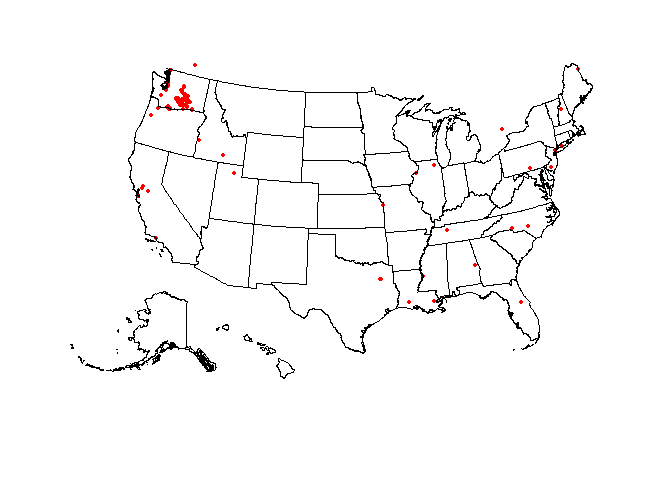
\includegraphics[width=1\linewidth]{Subquestions_files/figure-latex/user-map-us-1}

\begin{verbatim}
## 
## The downloaded binary packages are in
##  /var/folders/g8/z7k53ktx0pg62hb1c7cf4h1m0000gn/T//RtmpCSoUwV/downloaded_packages
\end{verbatim}

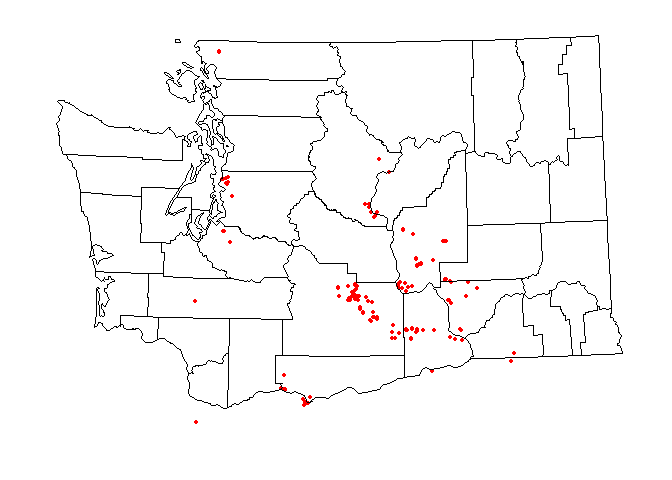
\includegraphics[width=1\linewidth]{Subquestions_files/figure-latex/user-map-wa-1}

\begin{verbatim}
## 
## The downloaded binary packages are in
##  /var/folders/g8/z7k53ktx0pg62hb1c7cf4h1m0000gn/T//RtmpCSoUwV/downloaded_packages
\end{verbatim}

\begin{verbatim}
##   |                                                                              |                                                                      |   0%  |                                                                              |=                                                                     |   1%  |                                                                              |=                                                                     |   2%  |                                                                              |==                                                                    |   2%  |                                                                              |==                                                                    |   3%  |                                                                              |===                                                                   |   4%  |                                                                              |===                                                                   |   5%  |                                                                              |====                                                                  |   5%  |                                                                              |====                                                                  |   6%  |                                                                              |=====                                                                 |   7%  |                                                                              |=====                                                                 |   8%  |                                                                              |======                                                                |   8%  |                                                                              |======                                                                |   9%  |                                                                              |=======                                                               |  10%  |                                                                              |=======                                                               |  11%  |                                                                              |========                                                              |  11%  |                                                                              |========                                                              |  12%  |                                                                              |=========                                                             |  13%  |                                                                              |==========                                                            |  14%  |                                                                              |==========                                                            |  15%  |                                                                              |===========                                                           |  15%  |                                                                              |===========                                                           |  16%  |                                                                              |============                                                          |  16%  |                                                                              |============                                                          |  17%  |                                                                              |============                                                          |  18%  |                                                                              |=============                                                         |  18%  |                                                                              |=============                                                         |  19%  |                                                                              |==============                                                        |  19%  |                                                                              |==============                                                        |  20%  |                                                                              |==============                                                        |  21%  |                                                                              |===============                                                       |  21%  |                                                                              |===============                                                       |  22%  |                                                                              |================                                                      |  22%  |                                                                              |================                                                      |  23%  |                                                                              |================                                                      |  24%  |                                                                              |=================                                                     |  24%  |                                                                              |=================                                                     |  25%  |                                                                              |==================                                                    |  25%  |                                                                              |==================                                                    |  26%  |                                                                              |===================                                                   |  27%  |                                                                              |====================                                                  |  28%  |                                                                              |====================                                                  |  29%  |                                                                              |=====================                                                 |  29%  |                                                                              |=====================                                                 |  30%  |                                                                              |======================                                                |  31%  |                                                                              |======================                                                |  32%  |                                                                              |=======================                                               |  32%  |                                                                              |=======================                                               |  33%  |                                                                              |========================                                              |  34%  |                                                                              |========================                                              |  35%  |                                                                              |=========================                                             |  35%  |                                                                              |=========================                                             |  36%  |                                                                              |==========================                                            |  37%  |                                                                              |==========================                                            |  38%  |                                                                              |===========================                                           |  38%  |                                                                              |===========================                                           |  39%  |                                                                              |============================                                          |  39%  |                                                                              |============================                                          |  40%  |                                                                              |=============================                                         |  41%  |                                                                              |=============================                                         |  42%  |                                                                              |==============================                                        |  43%  |                                                                              |===============================                                       |  44%  |                                                                              |===============================                                       |  45%  |                                                                              |================================                                      |  45%  |                                                                              |================================                                      |  46%  |                                                                              |=================================                                     |  47%  |                                                                              |=================================                                     |  48%  |                                                                              |==================================                                    |  48%  |                                                                              |==================================                                    |  49%  |                                                                              |===================================                                   |  49%  |                                                                              |===================================                                   |  50%  |                                                                              |===================================                                   |  51%  |                                                                              |====================================                                  |  51%  |                                                                              |====================================                                  |  52%  |                                                                              |=====================================                                 |  52%  |                                                                              |=====================================                                 |  53%  |                                                                              |======================================                                |  54%  |                                                                              |======================================                                |  55%  |                                                                              |=======================================                               |  55%  |                                                                              |=======================================                               |  56%  |                                                                              |========================================                              |  57%  |                                                                              |========================================                              |  58%  |                                                                              |=========================================                             |  58%  |                                                                              |=========================================                             |  59%  |                                                                              |==========================================                            |  60%  |                                                                              |===========================================                           |  61%  |                                                                              |===========================================                           |  62%  |                                                                              |============================================                          |  62%  |                                                                              |============================================                          |  63%  |                                                                              |=============================================                         |  64%  |                                                                              |=============================================                         |  65%  |                                                                              |==============================================                        |  65%  |                                                                              |==============================================                        |  66%  |                                                                              |===============================================                       |  66%  |                                                                              |===============================================                       |  67%  |                                                                              |===============================================                       |  68%  |                                                                              |================================================                      |  68%  |                                                                              |================================================                      |  69%  |                                                                              |=================================================                     |  69%  |                                                                              |=================================================                     |  70%  |                                                                              |=================================================                     |  71%  |                                                                              |==================================================                    |  71%  |                                                                              |==================================================                    |  72%  |                                                                              |===================================================                   |  72%  |                                                                              |===================================================                   |  73%  |                                                                              |====================================================                  |  74%  |                                                                              |====================================================                  |  75%  |                                                                              |=====================================================                 |  75%  |                                                                              |=====================================================                 |  76%  |                                                                              |======================================================                |  77%  |                                                                              |=======================================================               |  78%  |                                                                              |=======================================================               |  79%  |                                                                              |========================================================              |  79%  |                                                                              |========================================================              |  80%  |                                                                              |========================================================              |  81%  |                                                                              |=========================================================             |  81%  |                                                                              |=========================================================             |  82%  |                                                                              |==========================================================            |  82%  |                                                                              |==========================================================            |  83%  |                                                                              |===========================================================           |  84%  |                                                                              |===========================================================           |  85%  |                                                                              |============================================================          |  85%  |                                                                              |============================================================          |  86%  |                                                                              |=============================================================         |  87%  |                                                                              |=============================================================         |  88%  |                                                                              |==============================================================        |  88%  |                                                                              |==============================================================        |  89%  |                                                                              |===============================================================       |  90%  |                                                                              |================================================================      |  91%  |                                                                              |================================================================      |  92%  |                                                                              |=================================================================     |  92%  |                                                                              |=================================================================     |  93%  |                                                                              |=================================================================     |  94%  |                                                                              |==================================================================    |  94%  |                                                                              |==================================================================    |  95%  |                                                                              |===================================================================   |  95%  |                                                                              |===================================================================   |  96%  |                                                                              |====================================================================  |  97%  |                                                                              |====================================================================  |  98%  |                                                                              |===================================================================== |  98%  |                                                                              |===================================================================== |  99%  |                                                                              |======================================================================|  99%  |                                                                              |======================================================================| 100%
\end{verbatim}

\begin{verbatim}
##   |                                                                              |                                                                      |   0%  |                                                                              |                                                                      |   1%  |                                                                              |=                                                                     |   1%  |                                                                              |=                                                                     |   2%  |                                                                              |==                                                                    |   2%  |                                                                              |==                                                                    |   3%  |                                                                              |===                                                                   |   4%  |                                                                              |===                                                                   |   5%  |                                                                              |====                                                                  |   5%  |                                                                              |====                                                                  |   6%  |                                                                              |=====                                                                 |   7%  |                                                                              |=====                                                                 |   8%  |                                                                              |======                                                                |   8%  |                                                                              |======                                                                |   9%  |                                                                              |=======                                                               |   9%  |                                                                              |=======                                                               |  10%  |                                                                              |=======                                                               |  11%  |                                                                              |========                                                              |  11%  |                                                                              |========                                                              |  12%  |                                                                              |=========                                                             |  12%  |                                                                              |=========                                                             |  13%  |                                                                              |=========                                                             |  14%  |                                                                              |==========                                                            |  14%  |                                                                              |==========                                                            |  15%  |                                                                              |===========                                                           |  15%  |                                                                              |===========                                                           |  16%  |                                                                              |============                                                          |  16%  |                                                                              |============                                                          |  17%  |                                                                              |============                                                          |  18%  |                                                                              |=============                                                         |  18%  |                                                                              |=============                                                         |  19%  |                                                                              |==============                                                        |  19%  |                                                                              |==============                                                        |  20%  |                                                                              |==============                                                        |  21%  |                                                                              |===============                                                       |  21%  |                                                                              |===============                                                       |  22%  |                                                                              |================                                                      |  22%  |                                                                              |================                                                      |  23%  |                                                                              |=================                                                     |  24%  |                                                                              |=================                                                     |  25%  |                                                                              |==================                                                    |  25%  |                                                                              |==================                                                    |  26%  |                                                                              |===================                                                   |  27%  |                                                                              |===================                                                   |  28%  |                                                                              |====================                                                  |  28%  |                                                                              |====================                                                  |  29%  |                                                                              |=====================                                                 |  29%  |                                                                              |=====================                                                 |  30%  |                                                                              |=====================                                                 |  31%  |                                                                              |======================                                                |  31%  |                                                                              |======================                                                |  32%  |                                                                              |=======================                                               |  32%  |                                                                              |=======================                                               |  33%  |                                                                              |=======================                                               |  34%  |                                                                              |========================                                              |  34%  |                                                                              |========================                                              |  35%  |                                                                              |=========================                                             |  35%  |                                                                              |=========================                                             |  36%  |                                                                              |==========================                                            |  36%  |                                                                              |==========================                                            |  37%  |                                                                              |==========================                                            |  38%  |                                                                              |===========================                                           |  38%  |                                                                              |===========================                                           |  39%  |                                                                              |============================                                          |  39%  |                                                                              |============================                                          |  40%  |                                                                              |============================                                          |  41%  |                                                                              |=============================                                         |  41%  |                                                                              |=============================                                         |  42%  |                                                                              |==============================                                        |  42%  |                                                                              |==============================                                        |  43%  |                                                                              |===============================                                       |  44%  |                                                                              |===============================                                       |  45%  |                                                                              |================================                                      |  45%  |                                                                              |================================                                      |  46%  |                                                                              |=================================                                     |  46%  |                                                                              |=================================                                     |  47%  |                                                                              |=================================                                     |  48%  |                                                                              |==================================                                    |  48%  |                                                                              |==================================                                    |  49%  |                                                                              |===================================                                   |  49%  |                                                                              |===================================                                   |  50%  |                                                                              |===================================                                   |  51%  |                                                                              |====================================                                  |  51%  |                                                                              |====================================                                  |  52%  |                                                                              |=====================================                                 |  52%  |                                                                              |=====================================                                 |  53%  |                                                                              |=====================================                                 |  54%  |                                                                              |======================================                                |  54%  |                                                                              |======================================                                |  55%  |                                                                              |=======================================                               |  55%  |                                                                              |=======================================                               |  56%  |                                                                              |========================================                              |  57%  |                                                                              |========================================                              |  58%  |                                                                              |=========================================                             |  58%  |                                                                              |=========================================                             |  59%  |                                                                              |==========================================                            |  59%  |                                                                              |==========================================                            |  60%  |                                                                              |==========================================                            |  61%  |                                                                              |===========================================                           |  61%  |                                                                              |===========================================                           |  62%  |                                                                              |============================================                          |  62%  |                                                                              |============================================                          |  63%  |                                                                              |=============================================                         |  64%  |                                                                              |=============================================                         |  65%  |                                                                              |==============================================                        |  65%  |                                                                              |==============================================                        |  66%  |                                                                              |===============================================                       |  67%  |                                                                              |===============================================                       |  68%  |                                                                              |================================================                      |  68%  |                                                                              |================================================                      |  69%  |                                                                              |=================================================                     |  69%  |                                                                              |=================================================                     |  70%  |                                                                              |=================================================                     |  71%  |                                                                              |==================================================                    |  71%  |                                                                              |==================================================                    |  72%  |                                                                              |===================================================                   |  72%  |                                                                              |===================================================                   |  73%  |                                                                              |===================================================                   |  74%  |                                                                              |====================================================                  |  74%  |                                                                              |====================================================                  |  75%  |                                                                              |=====================================================                 |  75%  |                                                                              |=====================================================                 |  76%  |                                                                              |======================================================                |  76%  |                                                                              |======================================================                |  77%  |                                                                              |======================================================                |  78%  |                                                                              |=======================================================               |  78%  |                                                                              |=======================================================               |  79%  |                                                                              |========================================================              |  79%  |                                                                              |========================================================              |  80%  |                                                                              |========================================================              |  81%  |                                                                              |=========================================================             |  81%  |                                                                              |=========================================================             |  82%  |                                                                              |==========================================================            |  82%  |                                                                              |==========================================================            |  83%  |                                                                              |==========================================================            |  84%  |                                                                              |===========================================================           |  84%  |                                                                              |===========================================================           |  85%  |                                                                              |============================================================          |  85%  |                                                                              |============================================================          |  86%  |                                                                              |=============================================================         |  86%  |                                                                              |=============================================================         |  87%  |                                                                              |=============================================================         |  88%  |                                                                              |==============================================================        |  88%  |                                                                              |==============================================================        |  89%  |                                                                              |===============================================================       |  89%  |                                                                              |===============================================================       |  90%  |                                                                              |===============================================================       |  91%  |                                                                              |================================================================      |  91%  |                                                                              |================================================================      |  92%  |                                                                              |=================================================================     |  92%  |                                                                              |=================================================================     |  93%  |                                                                              |==================================================================    |  94%  |                                                                              |==================================================================    |  95%  |                                                                              |===================================================================   |  95%  |                                                                              |===================================================================   |  96%  |                                                                              |====================================================================  |  97%  |                                                                              |====================================================================  |  98%  |                                                                              |===================================================================== |  98%  |                                                                              |===================================================================== |  99%  |                                                                              |======================================================================|  99%  |                                                                              |======================================================================| 100%
\end{verbatim}

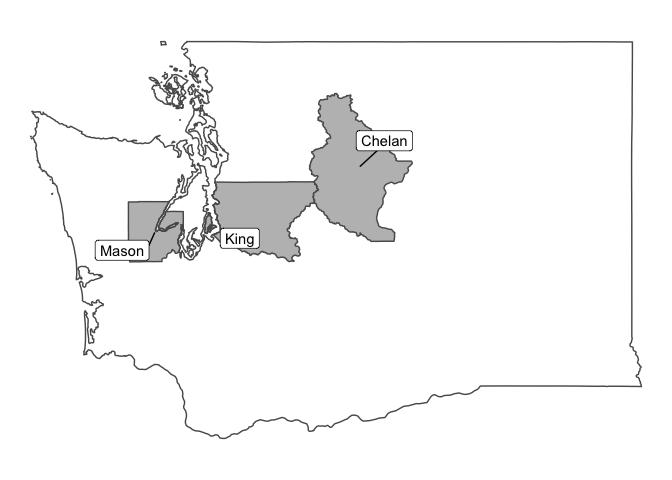
\includegraphics[width=1\linewidth]{Subquestions_files/figure-latex/user-map-wa-2}
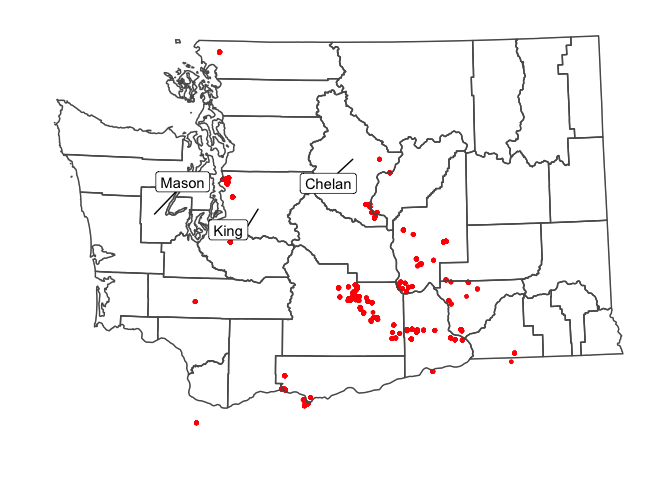
\includegraphics[width=1\linewidth]{Subquestions_files/figure-latex/user-map-wa-3}
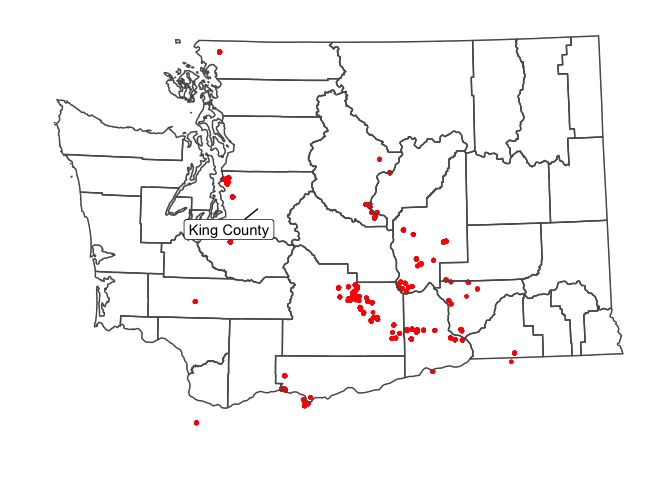
\includegraphics[width=1\linewidth]{Subquestions_files/figure-latex/user-map-wa-4}

\hypertarget{device-time-use-patterns}{%
\section{Device time use patterns}\label{device-time-use-patterns}}

\hypertarget{dataframe-summaries}{%
\section{Dataframe summaries}\label{dataframe-summaries}}

\begin{verbatim}
```r
# creating sessions 
# Goal: 1327 total sessions from 2020-08-26 through 2021-08-31. This doesn't include any sessions initiated by one of the 'ignored' aids.

install.packages("dplyr")
\end{verbatim}

\begin{verbatim}
## 
## The downloaded binary packages are in
##  /var/folders/g8/z7k53ktx0pg62hb1c7cf4h1m0000gn/T//RtmpCSoUwV/downloaded_packages
\end{verbatim}

\begin{Shaded}
\begin{Highlighting}[]
\FunctionTok{library}\NormalTok{(}\StringTok{"dplyr"}\NormalTok{)}
\FunctionTok{install.packages}\NormalTok{(}\StringTok{"lubridate"}\NormalTok{)}
\end{Highlighting}
\end{Shaded}

\begin{verbatim}
## 
## The downloaded binary packages are in
##  /var/folders/g8/z7k53ktx0pg62hb1c7cf4h1m0000gn/T//RtmpCSoUwV/downloaded_packages
\end{verbatim}

\begin{Shaded}
\begin{Highlighting}[]
\FunctionTok{library}\NormalTok{(}\StringTok{"lubridate"}\NormalTok{)}

\CommentTok{\#filter merged.csv from aid\textquotesingle{}s first "evStart" to the next "evStart"}
\NormalTok{merged.csv.dedup }\OtherTok{\textless{}{-}} \FunctionTok{unique}\NormalTok{(merged.csv)}

\NormalTok{x }\OtherTok{\textless{}{-}}\NormalTok{ merged.csv.dedup }\SpecialCharTok{\%\textgreater{}\%} 
  \FunctionTok{group\_by}\NormalTok{(}\AttributeTok{sessionid =} \FunctionTok{cumsum}\NormalTok{(evType }\SpecialCharTok{==} \StringTok{\textquotesingle{}evStart\textquotesingle{}}\NormalTok{)) }\SpecialCharTok{\%\textgreater{}\%} 
  \FunctionTok{mutate}\NormalTok{(}\AttributeTok{sessioneventno =} \FunctionTok{row\_number}\NormalTok{())}
\CommentTok{\# Problem with the code... look at line 1451, 1663 or 4052 (happens VERY rarely)}
\CommentTok{\# the code restarts the counter every time there is an evStart, however, if there are multiple users utilizing the app at the same time, the session ids and their actions are not distinguished }
\CommentTok{\# Solution: remove evType of statechange? I believe active{-}{-}\textgreater{}nonactive \& nonactive{-}{-}\textgreater{}active is ruining results... actually maybe not }

\NormalTok{x}\SpecialCharTok{$}\NormalTok{ts }\OtherTok{\textless{}{-}} \FunctionTok{ymd\_hms}\NormalTok{(x}\SpecialCharTok{$}\NormalTok{ts)}
\end{Highlighting}
\end{Shaded}

\begin{Shaded}
\begin{Highlighting}[]
\CommentTok{\# Objective: To understand the \textquotesingle{}Pesticide Labels Now\textquotesingle{} movile application user audience and their preferences for app utility. }

\CommentTok{\# Primary Research Question: How do user characteristics inform or explain their interaction with the \textquotesingle{}Pesticides Labels Now\textquotesingle{} application? }
\end{Highlighting}
\end{Shaded}

\begin{Shaded}
\begin{Highlighting}[]
\CommentTok{\# SubQuestion \#1: Which operating systems are utilized to access the application? }

\FunctionTok{str}\NormalTok{(evStart)}
\NormalTok{per\_data }\OtherTok{\textless{}{-}}\NormalTok{ evStart }\SpecialCharTok{\%\textgreater{}\%}
  \FunctionTok{count}\NormalTok{(device\_cat) }\SpecialCharTok{\%\textgreater{}\%} 
  \FunctionTok{mutate}\NormalTok{(}\AttributeTok{per =}\NormalTok{ n }\SpecialCharTok{/} \FunctionTok{sum}\NormalTok{(n),}
         \AttributeTok{per\_label =} \FunctionTok{paste0}\NormalTok{(}\FunctionTok{round}\NormalTok{(per}\SpecialCharTok{*}\DecValTok{100}\NormalTok{), }\StringTok{"\%"}\NormalTok{))}

\FunctionTok{ggplot}\NormalTok{(per\_data, }\FunctionTok{aes}\NormalTok{(}\AttributeTok{x =} \FunctionTok{reorder}\NormalTok{(n, }\SpecialCharTok{{-}}\NormalTok{per), }\AttributeTok{y=}\NormalTok{per)) }\SpecialCharTok{+} 
  \FunctionTok{geom\_bar}\NormalTok{(}\AttributeTok{stat =} \StringTok{"identity"}\NormalTok{, }\AttributeTok{fill =} \StringTok{"darkseagreen1"}\NormalTok{, }\AttributeTok{color =} \StringTok{"black"}\NormalTok{) }\SpecialCharTok{+} 
  \FunctionTok{geom\_text}\NormalTok{(}\FunctionTok{aes}\NormalTok{(}\AttributeTok{label=}\NormalTok{per\_label), }\AttributeTok{vjust=}\SpecialCharTok{{-}}\FloatTok{0.25}\NormalTok{) }\SpecialCharTok{+} 
  \FunctionTok{labs}\NormalTok{(}\AttributeTok{x =} \StringTok{"Devices"}\NormalTok{, }\AttributeTok{y =} \StringTok{"Count"}\NormalTok{,  }
       \AttributeTok{title =} \StringTok{"Operating Systems Utilized to Access the Application"}\NormalTok{) }\SpecialCharTok{+} 
  \FunctionTok{theme\_bw}\NormalTok{() }\SpecialCharTok{+} 
  \FunctionTok{scale\_x\_discrete}\NormalTok{(}\AttributeTok{labels =} \FunctionTok{c}\NormalTok{(}\StringTok{"iPhone"}\NormalTok{, }\StringTok{"Android"}\NormalTok{, }\StringTok{"iPad"}\NormalTok{, }\StringTok{"Pixel 3a: Android 10"}\NormalTok{))}
\end{Highlighting}
\end{Shaded}

\begin{Shaded}
\begin{Highlighting}[]
\CommentTok{\# SubQuestion \#2: Which language is more frequently utilized with the \textquotesingle{}Pesticide Labels Now\textquotesingle{} application? }

\FunctionTok{library}\NormalTok{(}\StringTok{"dplyr"}\NormalTok{)}
\NormalTok{count\_Language }\OtherTok{\textless{}{-}}\NormalTok{ evViewPage}\FloatTok{.01} \SpecialCharTok{\%\textgreater{}\%}
  \FunctionTok{count}\NormalTok{(evDesc2)}

\FunctionTok{library}\NormalTok{(tidyverse)}

\FunctionTok{str}\NormalTok{(evViewPage}\FloatTok{.01}\NormalTok{)}
\CommentTok{\#per\_data(2) \textless{}{-} evViewPage.01 \%\textgreater{}\%}
  \CommentTok{\#count(evDesc2) \%\textgreater{}\% }
  \CommentTok{\#mutate(per = n / sum(n),}
         \CommentTok{\#per\_label = paste0(round(per*100), "\%"))}

\FunctionTok{str}\NormalTok{(evStart)}
\NormalTok{per\_data }\OtherTok{\textless{}{-}}\NormalTok{ evStart }\SpecialCharTok{\%\textgreater{}\%}
  \FunctionTok{count}\NormalTok{(device\_cat) }\SpecialCharTok{\%\textgreater{}\%} 
  \FunctionTok{mutate}\NormalTok{(}\AttributeTok{per =}\NormalTok{ n }\SpecialCharTok{/} \FunctionTok{sum}\NormalTok{(n),}
         \AttributeTok{per\_label =} \FunctionTok{paste0}\NormalTok{(}\FunctionTok{round}\NormalTok{(per}\SpecialCharTok{*}\DecValTok{100}\NormalTok{), }\StringTok{"\%"}\NormalTok{))}

\FunctionTok{ggplot}\NormalTok{(per\_data, }\FunctionTok{aes}\NormalTok{(}\AttributeTok{x =} \FunctionTok{reorder}\NormalTok{(n, }\SpecialCharTok{{-}}\NormalTok{per), }\AttributeTok{y=}\NormalTok{per)) }\SpecialCharTok{+} 
  \FunctionTok{geom\_bar}\NormalTok{(}\AttributeTok{stat =} \StringTok{"identity"}\NormalTok{, }\AttributeTok{fill =} \StringTok{"lightblue"}\NormalTok{, }\AttributeTok{color =} \StringTok{"black"}\NormalTok{) }\SpecialCharTok{+} 
  \FunctionTok{geom\_text}\NormalTok{(}\FunctionTok{aes}\NormalTok{(}\AttributeTok{label=}\NormalTok{per\_label), }\AttributeTok{vjust=}\SpecialCharTok{{-}}\FloatTok{0.25}\NormalTok{) }\SpecialCharTok{+} 
  \FunctionTok{labs}\NormalTok{(}\AttributeTok{x =} \StringTok{"Language"}\NormalTok{, }\AttributeTok{y =} \StringTok{"Count"}\NormalTok{,  }
       \AttributeTok{title =} \StringTok{"Frequency of Each Language Accessed on the Application"}\NormalTok{) }\SpecialCharTok{+} 
  \FunctionTok{theme\_bw}\NormalTok{() }\SpecialCharTok{+} 
  \FunctionTok{scale\_x\_discrete}\NormalTok{(}\AttributeTok{labels =} \FunctionTok{c}\NormalTok{(}\StringTok{"English"}\NormalTok{, }\StringTok{"Spanish"}\NormalTok{))}
\end{Highlighting}
\end{Shaded}

\begin{Shaded}
\begin{Highlighting}[]
\CommentTok{\# Subquestion 1 + 2 Combined }

\FunctionTok{install.packages}\NormalTok{(}\StringTok{"tidyr"}\NormalTok{)}
\FunctionTok{library}\NormalTok{(tidyr)}

\NormalTok{device\_cat\_aid }\OtherTok{\textless{}{-}} \FunctionTok{unique}\NormalTok{(evStart[ , }\FunctionTok{c}\NormalTok{(}\StringTok{"aid"}\NormalTok{, }\StringTok{"device\_cat"}\NormalTok{)])}
\NormalTok{aid\_device\_language }\OtherTok{\textless{}{-}} \FunctionTok{left\_join}\NormalTok{(evViewPage}\FloatTok{.01}\NormalTok{, device\_cat\_aid, }\AttributeTok{by=}\StringTok{"aid"}\NormalTok{) }

\FunctionTok{table}\NormalTok{(aid\_device\_language}\SpecialCharTok{$}\NormalTok{evDesc2, aid\_device\_language}\SpecialCharTok{$}\NormalTok{device\_cat) }

\CommentTok{\#With percentage labels }
\CommentTok{\#https://stackoverflow.com/questions/68848650/create{-}percentage{-}labels{-}for{-}two{-}discrete{-}variables{-}in{-}ggplot{-}2}
\FunctionTok{ggplot}\NormalTok{(aid\_device\_language, }\FunctionTok{aes}\NormalTok{(}\AttributeTok{x=}\NormalTok{evDesc2)) }\SpecialCharTok{+} 
  \FunctionTok{geom\_bar}\NormalTok{(}\FunctionTok{aes}\NormalTok{(}\AttributeTok{y =} \DecValTok{2}\SpecialCharTok{*}\NormalTok{(..count..)}\SpecialCharTok{/}\FunctionTok{sum}\NormalTok{(..count..), }\AttributeTok{fill =}\NormalTok{ device\_cat, }\AttributeTok{group=}\NormalTok{device\_cat), }\AttributeTok{stat=}\StringTok{"count"}\NormalTok{) }\SpecialCharTok{+}
  \FunctionTok{geom\_label}\NormalTok{(}\FunctionTok{aes}\NormalTok{(}\AttributeTok{label =}\NormalTok{ scales}\SpecialCharTok{::}\FunctionTok{percent}\NormalTok{(}\DecValTok{2}\SpecialCharTok{*}\NormalTok{(..count..)}\SpecialCharTok{/}\FunctionTok{sum}\NormalTok{(..count..)),}
                  \AttributeTok{group =}\NormalTok{ device\_cat), }\AttributeTok{position =} \StringTok{"fill"}\NormalTok{, }\AttributeTok{stat=} \StringTok{"count"}\NormalTok{, }\AttributeTok{vjust =} \DecValTok{0}\NormalTok{) }\SpecialCharTok{+}
  \FunctionTok{labs}\NormalTok{(}\AttributeTok{y =} \StringTok{"Percent"}\NormalTok{, }\AttributeTok{fill=}\StringTok{"device\_cat"}\NormalTok{) }\SpecialCharTok{+}
  \FunctionTok{scale\_y\_continuous}\NormalTok{(}\AttributeTok{labels =}\NormalTok{ scales}\SpecialCharTok{::}\NormalTok{percent)}
  
\CommentTok{\#{-}{-}{-}{-}{-}{-}{-}{-}{-}{-}{-}{-}{-}{-}{-}{-}{-}{-}{-}{-}{-}{-}{-}{-}{-}{-}{-}{-}{-}{-}{-}{-}{-}{-}{-}{-}{-}{-}{-}{-}{-}{-}{-}{-}{-}{-}{-}{-}{-}{-}{-}{-}{-}{-}{-}{-}{-}{-}{-}{-}{-}{-}{-}{-}{-}{-}{-}{-}{-}{-}{-}{-}{-}{-}{-}{-}{-}{-}{-}{-}{-}{-}{-}{-}{-}{-}{-}{-}{-}{-}{-}{-}{-}{-}{-}{-}}

\CommentTok{\#Attempt 2: with percentage labels }
\FunctionTok{ggplot}\NormalTok{(}\AttributeTok{data =}\NormalTok{ aid\_device\_language2, }\AttributeTok{na.rm =} \ConstantTok{TRUE}\NormalTok{, }\FunctionTok{aes}\NormalTok{(}\AttributeTok{x =}\NormalTok{ evDesc2, }\AttributeTok{fill =}\NormalTok{ device\_cat)) }\SpecialCharTok{+} 
  \FunctionTok{geom\_bar}\NormalTok{(}\AttributeTok{position =} \StringTok{"fill"}\NormalTok{) }\SpecialCharTok{+} 
  \FunctionTok{scale\_y\_continuous}\NormalTok{(}\AttributeTok{labels =} \ControlFlowTok{function}\NormalTok{(x) }\FunctionTok{paste0}\NormalTok{(x}\SpecialCharTok{*}\DecValTok{100}\NormalTok{, }\StringTok{"\%"}\NormalTok{)) }\SpecialCharTok{+} 
   \FunctionTok{labs}\NormalTok{(}\AttributeTok{title =} \StringTok{"Frequency of Different Languages by Device"}\NormalTok{, }
       \AttributeTok{x =} \StringTok{"Language"}\NormalTok{, }
       \AttributeTok{y =} \StringTok{"Percentage"}\NormalTok{) }\SpecialCharTok{+}
      \FunctionTok{scale\_x\_discrete}\NormalTok{(}\AttributeTok{labels =} \FunctionTok{c}\NormalTok{(}\StringTok{"English"}\NormalTok{, }\StringTok{"Spanish"}\NormalTok{)) }\SpecialCharTok{+} 
      \FunctionTok{scale\_fill\_discrete}\NormalTok{(}\AttributeTok{name =} \StringTok{"Devices"}\NormalTok{, }\AttributeTok{labels =} \FunctionTok{c}\NormalTok{(}\StringTok{"Android"}\NormalTok{, }\StringTok{"iPad"}\NormalTok{, }\StringTok{"iPhone"}\NormalTok{,}\StringTok{"Pixel:Android 10"}\NormalTok{)) }\SpecialCharTok{+}     
        \FunctionTok{geom\_text}\NormalTok{(}\AttributeTok{data =}\NormalTok{ aid\_device\_language }\SpecialCharTok{\%\textgreater{}\%} 
              \FunctionTok{group\_by}\NormalTok{(evDesc2, device\_cat) }\SpecialCharTok{\%\textgreater{}\%}
              \FunctionTok{tally}\NormalTok{() }\SpecialCharTok{\%\textgreater{}\%}
              \FunctionTok{mutate}\NormalTok{(}\AttributeTok{p =}\NormalTok{ n }\SpecialCharTok{/} \FunctionTok{sum}\NormalTok{(n)) }\SpecialCharTok{\%\textgreater{}\%}
              \FunctionTok{ungroup}\NormalTok{(),}
            \FunctionTok{aes}\NormalTok{(}\AttributeTok{y =}\NormalTok{ p, }\AttributeTok{label =}\NormalTok{ scales}\SpecialCharTok{::}\FunctionTok{percent}\NormalTok{(p)),}
            \AttributeTok{position =} \FunctionTok{position\_stack}\NormalTok{(}\AttributeTok{vjust =} \FloatTok{0.5}\NormalTok{),}
            \AttributeTok{show.legend =} \ConstantTok{FALSE}\NormalTok{)}
            
\CommentTok{\#Option 1: figure how to add \textquotesingle{}Pixel 3a: Android 10\textquotesingle{} to android category }
\CommentTok{\# {-}{-} create a new variable}
\CommentTok{\# {-}{-} ggplot(ignore NA)}

\CommentTok{\#Option 2: Remove \textquotesingle{}Pixel 3a: Android 10\textquotesingle{} from dataset }
\CommentTok{\# Where is \textquotesingle{}NA\textquotesingle{} coming from? }

\CommentTok{\#{-}{-}{-}{-}{-}{-}{-}{-}{-}{-}{-}{-}{-}{-}{-}{-}{-}{-}{-}{-}{-}{-}{-}{-}{-}{-}{-}{-}{-}{-}{-}{-}{-}{-}{-}{-}{-}{-}{-}{-}{-}{-}{-}{-}{-}{-}{-}{-}{-}{-}{-}{-}{-}{-}{-}{-}{-}{-}{-}{-}{-}{-}{-}{-}{-}{-}{-}{-}{-}{-}{-}{-}{-}{-}{-}{-}{-}{-}{-}{-}{-}{-}{-}{-}{-}{-}{-}{-}{-}{-}{-}{-}{-}{-}{-}{-}}

\CommentTok{\#Without percentage labels }
\FunctionTok{install.packages}\NormalTok{(}\StringTok{"car"}\NormalTok{)}
\FunctionTok{library}\NormalTok{(car)}
\NormalTok{aid\_device\_language2 }\OtherTok{\textless{}{-}}\NormalTok{ aid\_device\_language}
\NormalTok{aid\_device\_language2}\SpecialCharTok{$}\NormalTok{device\_cat }\OtherTok{\textless{}{-}} \FunctionTok{recode}\NormalTok{(aid\_device\_language2}\SpecialCharTok{$}\NormalTok{device\_cat,}\StringTok{"c(\textquotesingle{}iphone\textquotesingle{}) = \textquotesingle{}iOS\textquotesingle{}"}\NormalTok{)}
\NormalTok{aid\_device\_language2}\SpecialCharTok{$}\NormalTok{device\_cat }\OtherTok{\textless{}{-}} \FunctionTok{recode}\NormalTok{(aid\_device\_language2}\SpecialCharTok{$}\NormalTok{device\_cat,}\StringTok{"c(\textquotesingle{}ipad\textquotesingle{}) = \textquotesingle{}iOS\textquotesingle{}"}\NormalTok{)}
\NormalTok{aid\_device\_language2}\SpecialCharTok{$}\NormalTok{device\_cat }\OtherTok{\textless{}{-}} \FunctionTok{recode}\NormalTok{(aid\_device\_language2}\SpecialCharTok{$}\NormalTok{device\_cat,}\StringTok{"c(\textquotesingle{}android\textquotesingle{}) = \textquotesingle{}Android\textquotesingle{}"}\NormalTok{)}
\NormalTok{aid\_device\_language2}\SpecialCharTok{$}\NormalTok{device\_cat }\OtherTok{\textless{}{-}} \FunctionTok{recode}\NormalTok{(aid\_device\_language2}\SpecialCharTok{$}\NormalTok{device\_cat,}\StringTok{"c(\textquotesingle{}Pixel 3a: Android 10\textquotesingle{}) = \textquotesingle{}android\textquotesingle{}"}\NormalTok{)}
\CommentTok{\#aid\_device\_language2$device\_cat \textless{}{-} case\_when(aid\_device\_language2$device\_cat == "Pixel 3a: Android 10" \textasciitilde{} "android", TRUE \textasciitilde{} NA)}

\NormalTok{aid\_device\_language2 }\OtherTok{\textless{}{-}} \FunctionTok{filter}\NormalTok{(aid\_device\_language2, }\SpecialCharTok{!}\FunctionTok{is.na}\NormalTok{(device\_cat))}

\NormalTok{aid\_device\_language2 }\OtherTok{\textless{}{-}} \FunctionTok{filter}\NormalTok{(aid\_device\_language2, }\SpecialCharTok{!}\FunctionTok{is.na}\NormalTok{(evDesc2))}

\FunctionTok{which}\NormalTok{(}\FunctionTok{is.na}\NormalTok{(aid\_device\_language2), }\AttributeTok{arr.ind=}\ConstantTok{TRUE}\NormalTok{)}


\FunctionTok{ggplot}\NormalTok{(}\AttributeTok{data =}\NormalTok{ aid\_device\_language2, }\FunctionTok{aes}\NormalTok{(}\AttributeTok{x =}\NormalTok{ evDesc2, }\AttributeTok{fill =}\NormalTok{ device\_cat)) }\SpecialCharTok{+} 
  \FunctionTok{geom\_bar}\NormalTok{(}\AttributeTok{position =} \StringTok{"fill"}\NormalTok{) }\SpecialCharTok{+} 
  \FunctionTok{scale\_y\_continuous}\NormalTok{(}\AttributeTok{labels =} \ControlFlowTok{function}\NormalTok{(x) }\FunctionTok{paste0}\NormalTok{(x}\SpecialCharTok{*}\DecValTok{100}\NormalTok{, }\StringTok{"\%"}\NormalTok{)) }\SpecialCharTok{+} 
   \FunctionTok{labs}\NormalTok{(}\AttributeTok{title =} \StringTok{"Frequency of Different Languages by Device"}\NormalTok{, }
       \AttributeTok{x =} \StringTok{"Language"}\NormalTok{, }
       \AttributeTok{y =} \StringTok{"Percentage"}\NormalTok{) }\SpecialCharTok{+}
      \FunctionTok{scale\_x\_discrete}\NormalTok{(}\AttributeTok{labels =} \FunctionTok{c}\NormalTok{(}\StringTok{"English"}\NormalTok{, }\StringTok{"Spanish"}\NormalTok{)) }\SpecialCharTok{+}
      \FunctionTok{scale\_fill\_discrete}\NormalTok{(}\AttributeTok{name =} \StringTok{"Operating System"}\NormalTok{, }\AttributeTok{labels =} \FunctionTok{c}\NormalTok{(}\StringTok{"Android"}\NormalTok{, }\StringTok{"iOS"}\NormalTok{))  }
\CommentTok{\#{-}{-}{-}{-}{-}{-}{-}{-}{-}{-}{-}{-}{-}{-}{-}{-}{-}{-}{-}{-}{-}{-}{-}{-}{-}{-}{-}{-}{-}{-}{-}{-}{-}{-}{-}{-}{-}{-}{-}{-}{-}{-}{-}{-}{-}{-}{-}{-}{-}{-}{-}{-}{-}{-}{-}{-}{-}{-}{-}{-}{-}{-}{-}{-}{-}{-}{-}{-}{-}{-}{-}{-}{-}{-}{-}{-}{-}{-}{-}{-}{-}{-}{-}{-}{-}{-}{-}{-}{-}{-}{-}{-}{-}{-}{-}{-}{-}{-}{-}{-}{-}{-}{-}      }
\FunctionTok{ggplot}\NormalTok{(}\AttributeTok{data =}\NormalTok{ aid\_device\_language2, }\FunctionTok{aes}\NormalTok{(}\AttributeTok{x =}\NormalTok{ evDesc2, }\AttributeTok{fill =}\NormalTok{ device\_cat)) }\SpecialCharTok{+} 
  \FunctionTok{geom\_bar}\NormalTok{(}\AttributeTok{position =} \StringTok{"fill"}\NormalTok{) }\SpecialCharTok{+} 
  \FunctionTok{scale\_y\_continuous}\NormalTok{(}\AttributeTok{labels =} \ControlFlowTok{function}\NormalTok{(x) }\FunctionTok{paste0}\NormalTok{(x}\SpecialCharTok{*}\DecValTok{100}\NormalTok{, }\StringTok{"\%"}\NormalTok{)) }\SpecialCharTok{+} 
   \FunctionTok{labs}\NormalTok{(}\AttributeTok{title =} \StringTok{"Frequency of Different Languages by Device"}\NormalTok{, }
       \AttributeTok{x =} \StringTok{"Language"}\NormalTok{, }
       \AttributeTok{y =} \StringTok{"Percentage"}\NormalTok{) }\SpecialCharTok{+}
      \FunctionTok{scale\_x\_discrete}\NormalTok{(}\AttributeTok{labels =} \FunctionTok{c}\NormalTok{(}\StringTok{"English"}\NormalTok{, }\StringTok{"Spanish"}\NormalTok{)) }\SpecialCharTok{+}
      \FunctionTok{scale\_fill\_discrete}\NormalTok{(}\AttributeTok{name =} \StringTok{"Operating System"}\NormalTok{, }\AttributeTok{labels =} \FunctionTok{c}\NormalTok{(}\StringTok{"Android"}\NormalTok{, }\StringTok{"iOS"}\NormalTok{)) }

\CommentTok{\#{-}{-}{-}{-}{-}{-}{-}{-}{-}{-}{-}{-}{-}{-}{-}{-}{-}{-}{-}{-}{-}{-}{-}{-}{-}{-}{-}{-}{-}{-}{-}{-}{-}{-}{-}{-}{-}{-}{-}{-}{-}{-}{-}{-}{-}{-}{-}{-}{-}{-}{-}{-}{-}{-}{-}{-}{-}{-}{-}{-}{-}{-}{-}{-}{-}{-}{-}{-}{-}{-}{-}{-}{-}{-}{-}{-}{-}{-}{-}{-}{-}{-}{-}{-}{-}{-}{-}{-}{-}{-}{-}{-}{-}{-}{-}{-}{-}{-}{-}{-}{-}{-}{-}}
\CommentTok{\#Original }
\FunctionTok{ggplot}\NormalTok{(}\AttributeTok{data =}\NormalTok{ aid\_device\_language, }\FunctionTok{aes}\NormalTok{(}\AttributeTok{x =}\NormalTok{ evDesc2, }\AttributeTok{fill =}\NormalTok{ device\_cat)) }\SpecialCharTok{+} 
  \FunctionTok{geom\_bar}\NormalTok{(}\AttributeTok{position =} \StringTok{"fill"}\NormalTok{) }\SpecialCharTok{+} 
  \FunctionTok{scale\_y\_continuous}\NormalTok{(}\AttributeTok{labels =} \ControlFlowTok{function}\NormalTok{(x) }\FunctionTok{paste0}\NormalTok{(x}\SpecialCharTok{*}\DecValTok{100}\NormalTok{, }\StringTok{"\%"}\NormalTok{)) }\SpecialCharTok{+} 
   \FunctionTok{labs}\NormalTok{(}\AttributeTok{title =} \StringTok{"Frequency of Different Languages by Device"}\NormalTok{, }
       \AttributeTok{x =} \StringTok{"Language"}\NormalTok{, }
       \AttributeTok{y =} \StringTok{"Percentage"}\NormalTok{) }\SpecialCharTok{+}
      \FunctionTok{scale\_x\_discrete}\NormalTok{(}\AttributeTok{labels =} \FunctionTok{c}\NormalTok{(}\StringTok{"English"}\NormalTok{, }\StringTok{"Spanish"}\NormalTok{)) }\SpecialCharTok{+} 
      \FunctionTok{scale\_fill\_discrete}\NormalTok{(}\AttributeTok{name =} \StringTok{"Devices"}\NormalTok{, }\AttributeTok{labels =} \FunctionTok{c}\NormalTok{(}\StringTok{"Android"}\NormalTok{, }\StringTok{"iPad"}\NormalTok{, }\StringTok{"iPhone"}\NormalTok{, }\StringTok{"Pixel 3a: Android 10"}\NormalTok{)) }
\end{Highlighting}
\end{Shaded}

\begin{Shaded}
\begin{Highlighting}[]
\CommentTok{\#Subquestion \#3: What is the relationship between location and utilization of the application? }

\FunctionTok{install.packages}\NormalTok{(}\StringTok{"usmap"}\NormalTok{)}
\FunctionTok{install.packages}\NormalTok{(}\StringTok{"ggplot2"}\NormalTok{)}

\CommentTok{\#evStart provides latitude and longitude of MOST USERS }
\CommentTok{\#1. remove variables that have "NA" for their latitude and longitude }
\NormalTok{evStart.location }\OtherTok{\textless{}{-}}\NormalTok{ evStart[}\SpecialCharTok{!}\NormalTok{(evStart}\SpecialCharTok{$}\NormalTok{lat}\SpecialCharTok{==}\StringTok{"n/a"} \SpecialCharTok{|}\NormalTok{ evStart}\SpecialCharTok{$}\NormalTok{lat}\SpecialCharTok{==}\StringTok{"NaN"}\NormalTok{),]}
\NormalTok{evStart.location}\FloatTok{.1} \OtherTok{\textless{}{-}} \FunctionTok{subset}\NormalTok{(evStart.location, }\AttributeTok{select =} \SpecialCharTok{{-}}\FunctionTok{c}\NormalTok{(aid, evDesc1, evDesc2, evDesc3, evType, ts, device\_cat))}


\CommentTok{\#interactive map? }
\FunctionTok{install.packages}\NormalTok{(}\StringTok{"leaflet"}\NormalTok{)}
\FunctionTok{install.packages}\NormalTok{(}\StringTok{"dplyr"}\NormalTok{)}

\FunctionTok{leaflet}\NormalTok{()}\SpecialCharTok{\%\textgreater{}\%}\FunctionTok{addTiles}\NormalTok{()}
\FunctionTok{leaflet}\NormalTok{()}\SpecialCharTok{\%\textgreater{}\%}\FunctionTok{addTiles}\NormalTok{()}\SpecialCharTok{\%\textgreater{}\%}\FunctionTok{addCircleMarkers}\NormalTok{(}\AttributeTok{data=}\NormalTok{evStart.location}\FloatTok{.1}\NormalTok{, }\AttributeTok{lat=} \SpecialCharTok{\textasciitilde{}}\NormalTok{lat, }\AttributeTok{lng =} \SpecialCharTok{\textasciitilde{}}\NormalTok{lon)}


\CommentTok{\# ERROR: "addCirclMarkers requires numeric longitude/latitude values" }

\CommentTok{\#{-}{-}{-}{-}{-}{-}{-}{-}{-}{-}{-}{-}{-}{-}{-}{-}{-}{-}{-}{-}{-}{-}{-}{-}{-}{-}{-}{-}{-}{-}{-}{-}{-}{-}{-}{-}{-}{-}{-}{-}{-}{-}{-}{-}{-}{-}{-}{-}{-}{-}{-}{-}{-}{-}{-}{-}{-}{-}{-}{-}{-}{-}{-}{-}{-}{-}{-}{-}{-}{-}{-}{-}{-}{-}{-}{-}{-}{-}{-}{-}{-}{-}{-}{-}{-}{-}{-}{-}{-}{-}{-}{-}{-}{-}{-}{-}{-}{-}{-}{-}{-}{-}{-}}

\CommentTok{\#united states map }
\FunctionTok{install.packages}\NormalTok{(}\StringTok{"usmap"}\NormalTok{)}
\FunctionTok{install.packages}\NormalTok{(}\StringTok{"maptools"}\NormalTok{)}
\FunctionTok{install.packages}\NormalTok{(}\StringTok{"rgdal"}\NormalTok{)}
\FunctionTok{library}\NormalTok{(maptools)}
\FunctionTok{library}\NormalTok{(}\StringTok{"rgdal"}\NormalTok{)}

\NormalTok{transformed\_data }\OtherTok{\textless{}{-}}  \FunctionTok{usmap\_transform}\NormalTok{(evStart.location}\FloatTok{.1}\NormalTok{)}

\FunctionTok{library}\NormalTok{(usmap)}
\FunctionTok{plot\_usmap}\NormalTok{(}\StringTok{"states"}\NormalTok{) }\SpecialCharTok{+} 
  \FunctionTok{geom\_point}\NormalTok{(}\AttributeTok{data =}\NormalTok{ transformed\_data, }
  \FunctionTok{aes}\NormalTok{(}\AttributeTok{x=}\NormalTok{lon}\FloatTok{.1}\NormalTok{, }\AttributeTok{y=}\NormalTok{lat}\FloatTok{.1}\NormalTok{),}
  \AttributeTok{color=}\StringTok{"red"}\NormalTok{,}
  \AttributeTok{size=}\DecValTok{3}\NormalTok{)}
\CommentTok{\# ERROR: "addCircleMarkers requires numeric longitude/latitude values" }
\end{Highlighting}
\end{Shaded}

\begin{Shaded}
\begin{Highlighting}[]
\CommentTok{\# Subquestion \#4: What is the average number of labels looked at per session? }

\CommentTok{\#Notes from Dennis on ‘How to find Number of Labels Search Per User in a Session’:}
\CommentTok{\# 1. Sort the list by aid }
\CommentTok{\# 2. Sort by time stamp (not that it matters)}
\CommentTok{\# 3. Iterate through the list from (1) evStart }
\CommentTok{\# 4. Set up a counter {-} evViewHS , from one evStart to the next evStart }
\end{Highlighting}
\end{Shaded}

\begin{Shaded}
\begin{Highlighting}[]
\CommentTok{\# Heatmap}
\FunctionTok{install.packages}\NormalTok{(}\StringTok{"data.table"}\NormalTok{)}
\end{Highlighting}
\end{Shaded}

\begin{verbatim}
## 
## The downloaded binary packages are in
##  /var/folders/g8/z7k53ktx0pg62hb1c7cf4h1m0000gn/T//RtmpCSoUwV/downloaded_packages
\end{verbatim}

\begin{Shaded}
\begin{Highlighting}[]
\FunctionTok{library}\NormalTok{(data.table)}
\end{Highlighting}
\end{Shaded}

\begin{verbatim}
## 
## Attaching package: 'data.table'
\end{verbatim}

\begin{verbatim}
## The following objects are masked from 'package:lubridate':
## 
##     hour, isoweek, mday, minute, month, quarter, second, wday, week,
##     yday, year
\end{verbatim}

\begin{verbatim}
## The following objects are masked from 'package:dplyr':
## 
##     between, first, last
\end{verbatim}

\begin{verbatim}
## The following object is masked from 'package:purrr':
## 
##     transpose
\end{verbatim}

\begin{Shaded}
\begin{Highlighting}[]
\FunctionTok{install.packages}\NormalTok{(}\StringTok{"dplyr"}\NormalTok{)}
\end{Highlighting}
\end{Shaded}

\begin{verbatim}
## 
## The downloaded binary packages are in
##  /var/folders/g8/z7k53ktx0pg62hb1c7cf4h1m0000gn/T//RtmpCSoUwV/downloaded_packages
\end{verbatim}

\begin{Shaded}
\begin{Highlighting}[]
\FunctionTok{library}\NormalTok{(dplyr)}
\FunctionTok{install.packages}\NormalTok{(}\StringTok{"ggplot2"}\NormalTok{)}
\end{Highlighting}
\end{Shaded}

\begin{verbatim}
## 
## The downloaded binary packages are in
##  /var/folders/g8/z7k53ktx0pg62hb1c7cf4h1m0000gn/T//RtmpCSoUwV/downloaded_packages
\end{verbatim}

\begin{Shaded}
\begin{Highlighting}[]
\FunctionTok{library}\NormalTok{(ggplot2)}
\FunctionTok{install.packages}\NormalTok{(}\StringTok{"lubridate"}\NormalTok{)}
\end{Highlighting}
\end{Shaded}

\begin{verbatim}
## 
## The downloaded binary packages are in
##  /var/folders/g8/z7k53ktx0pg62hb1c7cf4h1m0000gn/T//RtmpCSoUwV/downloaded_packages
\end{verbatim}

\begin{Shaded}
\begin{Highlighting}[]
\FunctionTok{library}\NormalTok{(lubridate)}

\FunctionTok{setDT}\NormalTok{(x)}
\NormalTok{y }\OtherTok{\textless{}{-}}\NormalTok{ x[ , .(}\AttributeTok{session\_start =} \FunctionTok{min}\NormalTok{(ts), }\AttributeTok{session\_end =} \FunctionTok{max}\NormalTok{(ts), }\AttributeTok{num\_occurance =}\NormalTok{ .N), by }\OtherTok{=}\NormalTok{ sessionid]}

\CommentTok{\#\textquotesingle{}session time\textquotesingle{} column is added }
\NormalTok{y}\SpecialCharTok{$}\NormalTok{sessiontime }\OtherTok{\textless{}{-}} \FunctionTok{ymd\_hms}\NormalTok{(y}\SpecialCharTok{$}\NormalTok{session\_end) }\SpecialCharTok{{-}} \FunctionTok{ymd\_hms}\NormalTok{(y}\SpecialCharTok{$}\NormalTok{session\_start)}
\NormalTok{y}\SpecialCharTok{$}\NormalTok{sessiontime2 }\OtherTok{\textless{}{-}} \FunctionTok{as.double}\NormalTok{(y}\SpecialCharTok{$}\NormalTok{sessiontime)}
\NormalTok{y}\SpecialCharTok{$}\NormalTok{sessiontimemin }\OtherTok{\textless{}{-}}\NormalTok{ y}\SpecialCharTok{$}\NormalTok{sessiontime2}\SpecialCharTok{/}\DecValTok{60}
\end{Highlighting}
\end{Shaded}

Time-Series Calendar HeatMap
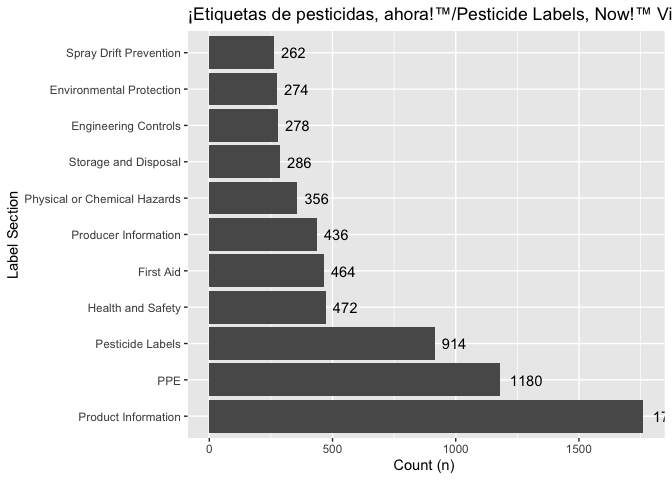
\includegraphics{Subquestions_files/figure-latex/unnamed-chunk-9-1.pdf}

\begin{Shaded}
\begin{Highlighting}[]
\CommentTok{\# heatmap attempt 4 (WORKS!)}
\CommentTok{\# x=hour of the day, y=day of the month, fill="activity"/number of occurances}
\FunctionTok{ggplot}\NormalTok{(y, }\FunctionTok{aes}\NormalTok{(}\AttributeTok{x=}\NormalTok{hour, }\AttributeTok{y=}\NormalTok{day)) }\SpecialCharTok{+} \FunctionTok{geom\_tile}\NormalTok{(}\FunctionTok{aes}\NormalTok{(}\AttributeTok{fill=}\NormalTok{num\_occurance)) }\SpecialCharTok{+}
  \FunctionTok{labs}\NormalTok{(}\AttributeTok{x=}\StringTok{"Hour of The Day"}\NormalTok{,}
       \AttributeTok{y=}\StringTok{"Day of the Month"}\NormalTok{,}
       \AttributeTok{title =} \StringTok{"Time{-}Series Calendar Heatmap"}\NormalTok{, }
       \AttributeTok{fill=}\StringTok{"Activity of the User"}\NormalTok{)}
\end{Highlighting}
\end{Shaded}

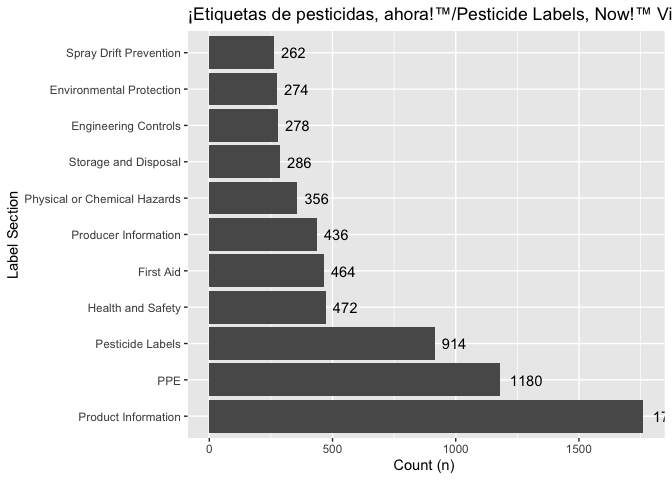
\includegraphics{Subquestions_files/figure-latex/unnamed-chunk-10-1.pdf}

\begin{Shaded}
\begin{Highlighting}[]
\CommentTok{\# heatmap attempt 6 (this is the one included in the poster)}
\CommentTok{\# sessiontime is done in seconds here }

\FunctionTok{ggplot}\NormalTok{(y, }\FunctionTok{aes}\NormalTok{(}\AttributeTok{x=}\NormalTok{day, }\AttributeTok{y=}\NormalTok{month)) }\SpecialCharTok{+} \FunctionTok{geom\_tile}\NormalTok{(}\FunctionTok{aes}\NormalTok{(}\AttributeTok{fill=}\NormalTok{sessiontimemin)) }\SpecialCharTok{+} 
\FunctionTok{scale\_y\_discrete}\NormalTok{(}\AttributeTok{limits =}\NormalTok{ month.abb) }\SpecialCharTok{+} 
 \FunctionTok{labs}\NormalTok{(}\AttributeTok{x=}\StringTok{"Day of the Month"}\NormalTok{,}
       \AttributeTok{y=}\StringTok{"Month"}\NormalTok{,}
       \AttributeTok{title =} \StringTok{"2020{-}2021 Calendar Heatmap"}\NormalTok{, }
       \AttributeTok{fill=}\StringTok{"Session Time (minutes)"}\NormalTok{)}
\end{Highlighting}
\end{Shaded}

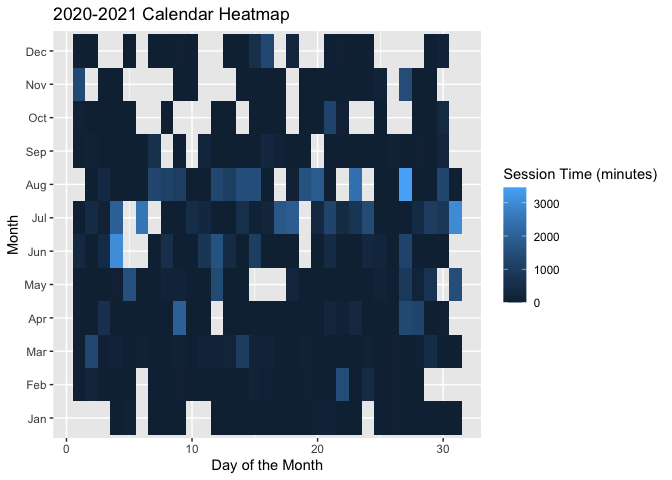
\includegraphics{Subquestions_files/figure-latex/unnamed-chunk-11-1.pdf}

\begin{Shaded}
\begin{Highlighting}[]
\CommentTok{\#heatmap attempt 7 (WORKS!)}
\CommentTok{\# (https://www.r{-}graph{-}gallery.com/283{-}the{-}hourly{-}heatmap.html)}
\CommentTok{\# Analyzes all 503 sessions... what day, time, and month }

\FunctionTok{install.packages}\NormalTok{(}\StringTok{"ggplot2"}\NormalTok{)}
\FunctionTok{library}\NormalTok{(ggplot2)}
\FunctionTok{install.packages}\NormalTok{(}\StringTok{"dplyr"}\NormalTok{)}
\FunctionTok{library}\NormalTok{(dplyr) }\CommentTok{\#easier data wrangling }
\FunctionTok{install.packages}\NormalTok{(}\StringTok{"viridis"}\NormalTok{)}
\FunctionTok{library}\NormalTok{(viridis) }\CommentTok{\#colour blind friendly palette, works in B\&W also}
\FunctionTok{install.packages}\NormalTok{(}\StringTok{"Interpol.T"}\NormalTok{)}
\FunctionTok{library}\NormalTok{(Interpol.T) }\CommentTok{\# will generate a large dataset on initial load}
\FunctionTok{install.packages}\NormalTok{(}\StringTok{"lubridate"}\NormalTok{)}
\FunctionTok{library}\NormalTok{(lubridate) }\CommentTok{\#for easy date manipulation}
\FunctionTok{install.packages}\NormalTok{(}\StringTok{"ggExtra"}\NormalTok{)}
\FunctionTok{library}\NormalTok{(ggExtra) }\CommentTok{\#because remembering ggplot theme options is beyond me}
\FunctionTok{install.packages}\NormalTok{(}\StringTok{"tidyr"}\NormalTok{)}
\FunctionTok{library}\NormalTok{(tidyr) }

\NormalTok{df }\OtherTok{\textless{}{-}}\NormalTok{y }\SpecialCharTok{\%\textgreater{}\%} \FunctionTok{select}\NormalTok{(sessionid,day,hour,month,year)}
\NormalTok{p }\OtherTok{\textless{}{-}}\FunctionTok{ggplot}\NormalTok{(df,}\FunctionTok{aes}\NormalTok{(day,hour))}\SpecialCharTok{+}
  \FunctionTok{geom\_tile}\NormalTok{(}\AttributeTok{color=} \StringTok{"white"}\NormalTok{,}\AttributeTok{size=}\FloatTok{0.1}\NormalTok{) }\SpecialCharTok{+} 
  \FunctionTok{scale\_fill\_viridis}\NormalTok{(}\AttributeTok{name=}\StringTok{"Hrly Temps C"}\NormalTok{,}\AttributeTok{option =}\StringTok{"C"}\NormalTok{)}
\NormalTok{p }\OtherTok{\textless{}{-}}\NormalTok{p }\SpecialCharTok{+} \FunctionTok{facet\_grid}\NormalTok{(year}\SpecialCharTok{\textasciitilde{}}\NormalTok{month)}
\NormalTok{p }\OtherTok{\textless{}{-}}\NormalTok{p }\SpecialCharTok{+} \FunctionTok{scale\_y\_continuous}\NormalTok{(}\AttributeTok{trans =} \StringTok{"reverse"}\NormalTok{, }\AttributeTok{breaks =} \FunctionTok{unique}\NormalTok{(df}\SpecialCharTok{$}\NormalTok{hour))}
\NormalTok{p }\OtherTok{\textless{}{-}}\NormalTok{p }\SpecialCharTok{+} \FunctionTok{scale\_x\_continuous}\NormalTok{(}\AttributeTok{breaks =}\FunctionTok{c}\NormalTok{(}\DecValTok{1}\NormalTok{,}\DecValTok{10}\NormalTok{,}\DecValTok{20}\NormalTok{,}\DecValTok{31}\NormalTok{))}
\NormalTok{p }\OtherTok{\textless{}{-}}\NormalTok{p }\SpecialCharTok{+} \FunctionTok{theme\_minimal}\NormalTok{(}\AttributeTok{base\_size =} \DecValTok{8}\NormalTok{)}
\NormalTok{p }\OtherTok{\textless{}{-}}\NormalTok{p }\SpecialCharTok{+} \FunctionTok{labs}\NormalTok{(}\AttributeTok{title=} \FunctionTok{paste}\NormalTok{(}\StringTok{"Session Analytics"}\NormalTok{), }\AttributeTok{x=}\StringTok{"Day of the Month"}\NormalTok{, }\AttributeTok{y=}\StringTok{"Hour Commencing"}\NormalTok{)}
\NormalTok{p }\OtherTok{\textless{}{-}}\NormalTok{p }\SpecialCharTok{+} \FunctionTok{theme}\NormalTok{(}\AttributeTok{legend.position =} \StringTok{"bottom"}\NormalTok{)}\SpecialCharTok{+}
  \FunctionTok{theme}\NormalTok{(}\AttributeTok{plot.title=}\FunctionTok{element\_text}\NormalTok{(}\AttributeTok{size =} \DecValTok{14}\NormalTok{))}\SpecialCharTok{+}
  \FunctionTok{theme}\NormalTok{(}\AttributeTok{axis.text.y=}\FunctionTok{element\_text}\NormalTok{(}\AttributeTok{size=}\DecValTok{6}\NormalTok{)) }\SpecialCharTok{+}
  \FunctionTok{theme}\NormalTok{(}\AttributeTok{strip.background =} \FunctionTok{element\_rect}\NormalTok{(}\AttributeTok{colour=}\StringTok{"white"}\NormalTok{))}\SpecialCharTok{+}
  \FunctionTok{theme}\NormalTok{(}\AttributeTok{plot.title=}\FunctionTok{element\_text}\NormalTok{(}\AttributeTok{hjust=}\DecValTok{0}\NormalTok{))}\SpecialCharTok{+}
  \FunctionTok{theme}\NormalTok{(}\AttributeTok{axis.ticks=}\FunctionTok{element\_blank}\NormalTok{())}\SpecialCharTok{+}
  \FunctionTok{theme}\NormalTok{(}\AttributeTok{axis.text=}\FunctionTok{element\_text}\NormalTok{(}\AttributeTok{size=}\DecValTok{7}\NormalTok{))}\SpecialCharTok{+}
  \FunctionTok{theme}\NormalTok{(}\AttributeTok{legend.title=}\FunctionTok{element\_text}\NormalTok{(}\AttributeTok{size=}\DecValTok{8}\NormalTok{))}\SpecialCharTok{+}
  \FunctionTok{theme}\NormalTok{(}\AttributeTok{legend.text=}\FunctionTok{element\_text}\NormalTok{(}\AttributeTok{size=}\DecValTok{6}\NormalTok{))}
\NormalTok{p}
\end{Highlighting}
\end{Shaded}

\begin{Shaded}
\begin{Highlighting}[]
\CommentTok{\# heatmap attempt }
\FunctionTok{install.packages}\NormalTok{(}\StringTok{"ggplot2"}\NormalTok{)}
\FunctionTok{library}\NormalTok{(ggplot2)}
\FunctionTok{install.packages}\NormalTok{(}\StringTok{"dplyr"}\NormalTok{)}
\FunctionTok{library}\NormalTok{(dplyr) }\CommentTok{\#easier data wrangling }
\FunctionTok{install.packages}\NormalTok{(}\StringTok{"viridis"}\NormalTok{)}
\FunctionTok{library}\NormalTok{(viridis) }\CommentTok{\#colour blind friendly palette, works in B\&W also}
\FunctionTok{install.packages}\NormalTok{(}\StringTok{"Interpol.T"}\NormalTok{)}
\FunctionTok{library}\NormalTok{(Interpol.T) }\CommentTok{\# will generate a large dataset on initial load}
\FunctionTok{install.packages}\NormalTok{(}\StringTok{"lubridate"}\NormalTok{)}
\FunctionTok{library}\NormalTok{(lubridate) }\CommentTok{\#for easy date manipulation}
\FunctionTok{install.packages}\NormalTok{(}\StringTok{"ggExtra"}\NormalTok{)}
\FunctionTok{library}\NormalTok{(ggExtra) }\CommentTok{\#because remembering ggplot theme options is beyond me}
\FunctionTok{install.packages}\NormalTok{(}\StringTok{"tidyr"}\NormalTok{)}
\FunctionTok{library}\NormalTok{(tidyr) }

\NormalTok{df }\OtherTok{\textless{}{-}}\NormalTok{y }\SpecialCharTok{\%\textgreater{}\%} \FunctionTok{select}\NormalTok{(sessionid,day,hour,month,year) }\SpecialCharTok{\%\textgreater{}\%} \FunctionTok{fill}\NormalTok{(sessiontime2)}
\NormalTok{p }\OtherTok{\textless{}{-}}\FunctionTok{ggplot}\NormalTok{(df,}\FunctionTok{aes}\NormalTok{(day,hour, }\AttributeTok{fill=}\NormalTok{sessiontime2))}\SpecialCharTok{+}
  \FunctionTok{geom\_tile}\NormalTok{(}\AttributeTok{color=} \StringTok{"white"}\NormalTok{,}\AttributeTok{size=}\FloatTok{0.1}\NormalTok{) }\SpecialCharTok{+} 
  \FunctionTok{scale\_fill\_viridis}\NormalTok{(}\AttributeTok{name=}\StringTok{"Hrly Temps C"}\NormalTok{,}\AttributeTok{option =}\StringTok{"C"}\NormalTok{)}
\NormalTok{p }\OtherTok{\textless{}{-}}\NormalTok{p }\SpecialCharTok{+} \FunctionTok{facet\_grid}\NormalTok{(year}\SpecialCharTok{\textasciitilde{}}\NormalTok{month)}
\NormalTok{p }\OtherTok{\textless{}{-}}\NormalTok{p }\SpecialCharTok{+} \FunctionTok{scale\_y\_continuous}\NormalTok{(}\AttributeTok{trans =} \StringTok{"reverse"}\NormalTok{, }\AttributeTok{breaks =} \FunctionTok{unique}\NormalTok{(df}\SpecialCharTok{$}\NormalTok{hour))}
\NormalTok{p }\OtherTok{\textless{}{-}}\NormalTok{p }\SpecialCharTok{+} \FunctionTok{scale\_x\_continuous}\NormalTok{(}\AttributeTok{breaks =}\FunctionTok{c}\NormalTok{(}\DecValTok{1}\NormalTok{,}\DecValTok{10}\NormalTok{,}\DecValTok{20}\NormalTok{,}\DecValTok{31}\NormalTok{))}
\NormalTok{p }\OtherTok{\textless{}{-}}\NormalTok{p }\SpecialCharTok{+} \FunctionTok{theme\_minimal}\NormalTok{(}\AttributeTok{base\_size =} \DecValTok{8}\NormalTok{)}
\NormalTok{p }\OtherTok{\textless{}{-}}\NormalTok{p }\SpecialCharTok{+} \FunctionTok{labs}\NormalTok{(}\AttributeTok{title=} \FunctionTok{paste}\NormalTok{(}\StringTok{"Session Analytics"}\NormalTok{), }\AttributeTok{x=}\StringTok{"Day of the Month"}\NormalTok{, }\AttributeTok{y=}\StringTok{"Hour Commencing"}\NormalTok{)}
\NormalTok{p }\OtherTok{\textless{}{-}}\NormalTok{p }\SpecialCharTok{+} \FunctionTok{theme}\NormalTok{(}\AttributeTok{legend.position =} \StringTok{"bottom"}\NormalTok{)}\SpecialCharTok{+}
  \FunctionTok{theme}\NormalTok{(}\AttributeTok{plot.title=}\FunctionTok{element\_text}\NormalTok{(}\AttributeTok{size =} \DecValTok{14}\NormalTok{))}\SpecialCharTok{+}
  \FunctionTok{theme}\NormalTok{(}\AttributeTok{axis.text.y=}\FunctionTok{element\_text}\NormalTok{(}\AttributeTok{size=}\DecValTok{6}\NormalTok{)) }\SpecialCharTok{+}
  \FunctionTok{theme}\NormalTok{(}\AttributeTok{strip.background =} \FunctionTok{element\_rect}\NormalTok{(}\AttributeTok{colour=}\StringTok{"white"}\NormalTok{))}\SpecialCharTok{+}
  \FunctionTok{theme}\NormalTok{(}\AttributeTok{plot.title=}\FunctionTok{element\_text}\NormalTok{(}\AttributeTok{hjust=}\DecValTok{0}\NormalTok{))}\SpecialCharTok{+}
  \FunctionTok{theme}\NormalTok{(}\AttributeTok{axis.ticks=}\FunctionTok{element\_blank}\NormalTok{())}\SpecialCharTok{+}
  \FunctionTok{theme}\NormalTok{(}\AttributeTok{axis.text=}\FunctionTok{element\_text}\NormalTok{(}\AttributeTok{size=}\DecValTok{7}\NormalTok{))}\SpecialCharTok{+}
  \FunctionTok{theme}\NormalTok{(}\AttributeTok{legend.title=}\FunctionTok{element\_text}\NormalTok{(}\AttributeTok{size=}\DecValTok{8}\NormalTok{))}\SpecialCharTok{+}
  \FunctionTok{theme}\NormalTok{(}\AttributeTok{legend.text=}\FunctionTok{element\_text}\NormalTok{(}\AttributeTok{size=}\DecValTok{6}\NormalTok{))}
\NormalTok{p}
\end{Highlighting}
\end{Shaded}

\begin{Shaded}
\begin{Highlighting}[]
\CommentTok{\# cumulative distribution plot}
\CommentTok{\# https://rpubs.com/tgjohnst/cumulative\_plotting}
\CommentTok{\# https://stackoverflow.com/questions/66471218/plotting{-}a{-}cumulative{-}frequency{-}curve{-}on{-}a{-}histogram{-}in{-}r}
\end{Highlighting}
\end{Shaded}

\begin{Shaded}
\begin{Highlighting}[]
\CommentTok{\# Average session duration }
\FunctionTok{sum}\NormalTok{(y}\SpecialCharTok{$}\NormalTok{sessiontime)}
\end{Highlighting}
\end{Shaded}

\begin{verbatim}
## Time difference of 7179658 secs
\end{verbatim}

\begin{Shaded}
\begin{Highlighting}[]
\NormalTok{(}\DecValTok{7179658}\SpecialCharTok{/}\DecValTok{60}\NormalTok{)}
\end{Highlighting}
\end{Shaded}

\begin{verbatim}
## [1] 119661
\end{verbatim}

\begin{Shaded}
\begin{Highlighting}[]
\DecValTok{119661}\SpecialCharTok{/}\DecValTok{1328}
\end{Highlighting}
\end{Shaded}

\begin{verbatim}
## [1] 90.10617
\end{verbatim}

\begin{Shaded}
\begin{Highlighting}[]
\CommentTok{\#90.11}
\end{Highlighting}
\end{Shaded}

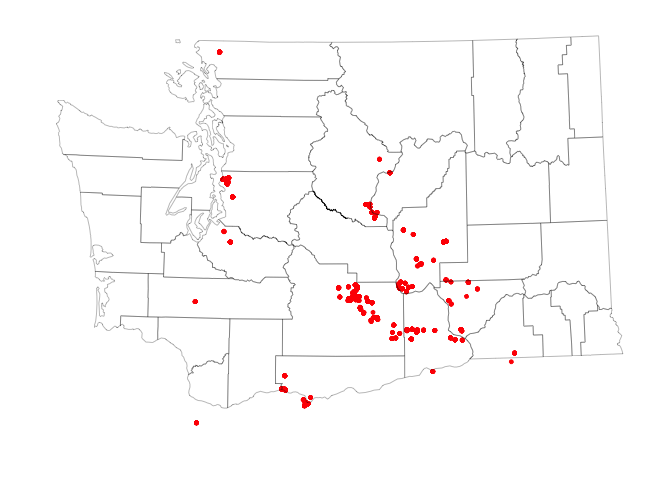
\includegraphics[width=1\linewidth]{Subquestions_files/figure-latex/user-map-wa-2-1}

\end{document}
